\documentclass[a4paper]{article}

\usepackage[english]{babel}
\usepackage[utf8]{inputenc}
\usepackage{amsmath}
\usepackage{graphicx}
\usepackage[colorinlistoftodos]{todonotes}
% \usepackage{comment}


%TODO

% Add background concepts
% Add table for balanced ternary
%	use as an intro to probability current
% Physical Implementations
% Brief discussion of the different archetectures
% Discuss access of machines themselves
% Discuss how to use code API such as QiSkit


\title{A Brief introduction to Quantum Computing from the Perspective of Ladder Logic}

\author{Jerry Kensler}

\date{\today}

\begin{document}
\maketitle

\begin{abstract}
	
	%Reword this, it's  too boring
	
%Enter a short summary here. What topic do you want to investigate and why? What experiment did you perform? What were your main results and conclusion?
%

%Quantum computing, for several years the media and public perception of the subject has treated it akin to magic, using it as a catchall for any science fiction plot device deemed necessary.  Because of this, otherwise capable individuals may tend to stray away from the subject purely due to its perceived difficulty, many assuming they would need doctorates to even begin to comprehend the complexities of quantum computing.  Indeed, quantum physics is very complex, having many important real-world ramifications. With that said, quantum computing is merely a small part of quantum physics, and much like the computing most people use daily, operates by a well-defined set of rules.  By utilizing a subset of these rules, specifically tools such as quantum ladder logic, quantum assembly (QASM), and visual aids such as Bloch spheres, much of the initial barrier to entry can be circumvented.  While this approach isn’t perfect, and will require more serious individuals to pursue much of the background math and physics on their own.  It is my hope that students, specifically those with a background in electronic circuits and/or programming will find the contents of this paper able to greatly reduce the amount of time and effort needed in order to start learning how to program a quantum computer and thus prepare themselves for a future where such technology is prevalent.

Insert Better Version of introduction here.  Didn't Like the original one.

Keywords:  Quantum, QISKit, Computing, Ladder, Logic, QASM, Introduction
% Need to reword this section, Find the abstract from source and merge the two
% Author note: the intention of this paper is to fill some of the skill gap many novices encounter in learning quantum computing.  By no means should this be considered an all-encompassing guide to the subject matter.
\end{abstract}




\section{Introduction 5 lines to max 1/2 page}
\label{sec:introduction}

%Explain the context of the experiment here. Why is condensed matter physics interesting or important?
%Optional things you could talk about (but don't have to -- this is up to you): transistors, computers, Quantum computers, fundamental knowledge (e.g. the resistance quantum).

%Briefly explain what methods you will use in the experiment, and what values you will extract from the data.

%For this section and all following sections: If you refer to an equation, previous result or theory that is not regarded as common knowledge, then cite the source (article or book) where you found this. For example, you can cite the Nano 3 Lecture notes \cite{nano3}.

This section is for context.  The how, and why.  From here on out, if I refer to a theory that isn't common knowledge, cite the source. \cite{junctNew}.


\section{Background Concepts}
\label{sec:backgroundconcepts}
%brief intro to this section, needs rewording
This section is not meant to be an exhaustive list, but, in my personal experience, learning about the background concepts below will greatly assist a person’s ability to better understand quantum computing.  The following sections will provide a brief explanation of the concepts.
\subsection{Balanced Ternary} %The basics from the ground up
%note: blanaced ternary is not, strictly speaking a core mechanic in quantum computing.  However, it could serve as a gentle introduction to non-binary coding for many students.  A bridge between hard digital and the strangeness of qubits
insert balanced ternary section here along with comparison table.

%\subsection{How to Make Tables}

Use the table and tabular commands for basic tables --- see Table~\ref{tab:widgets}, for example.

\begin{table}
	\centering
	\begin{tabular}{l|l|l} % Justification l-left, c-center, r-right
		Decimal & Binary (IEEE 754*) & Balanced Ternary \\\hline
		0 & 0 & 0 \\
		3 & 11 & 10 \\
		5 & 101 & + 0 - \\
		-254 & 11000011011111100000000000000000* & - 0 0 - + - \\ % -3^5 + 0 + 0 - 3^2 + 3^1 -3^0
	\end{tabular}
	\caption{\label{tab:widgets}comparison table showing equivalent numbers in different display forms}
\end{table}


\subsection{Reversible Logic Gates} %The basics from the ground up
%there was a time when reversible logic was seen as a fatal flaw in QC, but some dude who was pretty clever figured out any standard logic gate could be simulated within reversible logic
Talk about why reversible logic gates are important to quantum computing, a bit of the history, etc.


\section{Theory 2-3 pages}
\label{sec:theory}

\subsection{Two-dimensional Electron Gas}
Here, explain the concept of a 2-DEG in GaAs/AlGaAs. What is a 2-DEG and why does it arise?

\subsection{Hall Effect}
Explain the classical Hall effect in your own words. What do I measure at $B=0$? And what happens if $B>0$? Which effect gives rise to the voltage drop in the vertical direction?

\subsection{Quantum Hall Effect}
Explain the IQHE in your own words. What does the density of states look like in a 2-DEG when $B=0$? What are Landau levels and how do they arise? What are edge states? What does the electron transport look like when you change the magnetic field? What do you expect to measure?

\section{Experiment 1-2 pages}
\subsection{Fabrication}
Explain a step-by-step recipe for fabrication here. How long did you etch and why? What is an Ohmic contact?
\subsection{Experimental set-up}
Explain the experimental set-up here. Use a schematic picture (make it yourself in photoshop, paint, ...) to show how the components are connected. Briefly explain how a lock-in amplifier works.

\section{Results and interpretation 2-3 pages}
Show a graph of the longitudinal resistivity ($\rho_{xx}$) and Hall resistivity ($\rho_{xy}$) versus magnetic field, extracted from the raw data shown in figure \ref{fig:data}. You will have the link to the data in your absalon messages, if not e-mail Guen (guen@nbi.dk). Explain how you calculated these values, and refer to the theory.

%\begin{figure}
%\centering
%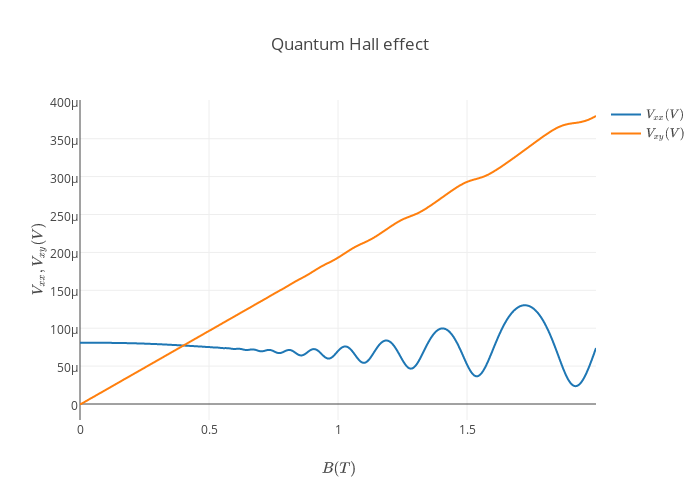
\includegraphics[width=1\textwidth]{raw_data.png}
%\caption{\label{fig:data}Raw (unprocessed) data. Replace this %figure %with the one you've made, that shows the resistivity.}
%\end{figure}

\subsection{Classical regime}
Calculate the sheet electron density $n_{s}$ and electron mobility $\mu$ from the data in the low-field regime, and refer to the theory in section \ref{sec:theory}. Explain how you retrieved the values from the data (did you use a linear fit?).
Round values off to 1 or 2 significant digits: 8.1643 ~= 8.2. Also, 5e-6 is easier to read than 0.000005.

!OBS: This part is optional (only if you have time left).
Calculate the uncertainty as follows: \newline $u(f(x, y, z)) = \sqrt{(\frac{\delta f}{\delta{x}} u(x))^{2} + (\frac{\delta f}{\delta{y}} u(y))^{2} + (\frac{\delta f}{\delta{z}} u(z))^{2}}$, where $f$ is the calculated value ($n_{s}$ or $\mu$), $x, y, z$ are the variables taken from the measurement and $u(x)$ is the uncertainty in x (and so on).

\subsection{Quantum regime}
Calculate $n_{s}$ for the high-field regime.
Show a graph of the longitudinal conductivity ($\rho_{xx}$) and Hall conductivity($\rho_{xy}$) \textbf{in units of the resistance quantum} ($\frac{h}{e^{2}}$), depicting the integer filling factors for each plateau.
Show a graph of the plateau number versus its corresponding value of $1/B$. From this you can determine the slope, which you use to calculate the electron density.
Again, calculate the uncertainty for your obtained values.

\section{Discussion 1/2-1 page}
Discuss your results. Compare the two values of $n_{s}$ that you've found in the previous section. Compare your results with literature and comment on the difference. If you didn't know the value of the resistance quantum, would you be able to deduce it from your measurements? If yes/no, why?

\newpage
\section{Some LaTeX tips}
\label{sec:latex}
\subsection{How to Include Figures}

First you have to upload the image file (JPEG, PNG or PDF) from your computer to writeLaTeX using the upload link the project menu. Then use the includegraphics command to include it in your document. Use the figure environment and the caption command to add a number and a caption to your figure. See the code for Figure \ref{fig:frog} in this section for an example.

%\begin{figure}
%\centering
%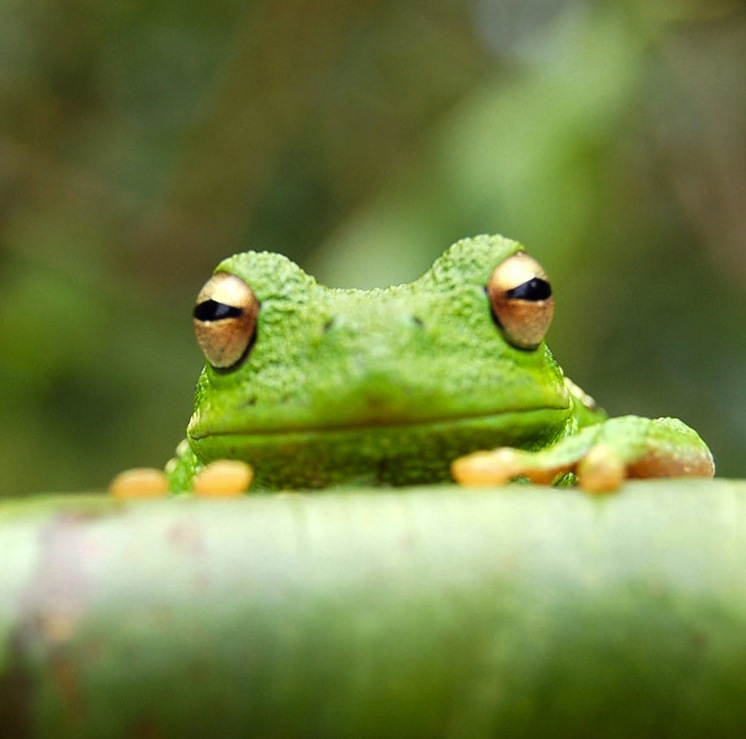
\includegraphics[width=0.3\textwidth]{frog.jpg}
%\caption{\label{fig:frog}This frog was uploaded to writeLaTeX via %the project menu.}
%\end{figure}



\subsection{How to Write Mathematics}

\LaTeX{} is great at typesetting mathematics. Let $X_1, X_2, \ldots, X_n$ be a sequence of independent and identically distributed random variables with $\text{E}[X_i] = \mu$ and $\text{Var}[X_i] = \sigma^2 < \infty$, and let

\begin{equation}
S_n = \frac{X_1 + X_2 + \cdots + X_n}{n}
      = \frac{1}{n}\sum_{i}^{n} X_i
\label{eq:sn}
\end{equation}

denote their mean. Then as $n$ approaches infinity, the random variables $\sqrt{n}(S_n - \mu)$ converge in distribution to a normal $\mathcal{N}(0, \sigma^2)$.

The equation \ref{eq:sn} is very nice.

\subsection{How to Make Sections and Subsections}

Use section and subsection commands to organize your document. \LaTeX{} handles all the formatting and numbering automatically. Use ref and label commands for cross-references.

\subsection{How to Make Lists}

You can make lists with automatic numbering \dots

\begin{enumerate}
\item Like this,
\item and like this.
\end{enumerate}
\dots or bullet points \dots
\begin{itemize}
\item Like this,
\item and like this.
\end{itemize}
\dots or with words and descriptions \dots
\begin{description}
\item[Word] Definition
\item[Concept] Explanation
\item[Idea] Text
\end{description}

We hope you find write\LaTeX\ useful, and please let us know if you have any feedback using the help menu above.

\begin{thebibliography}{9}
	
	%Begin Original Text, keeping for referece========================
	
% \bibitem{nano3}
% 	K. Grove-Rasmussen og Jesper Nygård,
%  	\emph{Kvantefænomener i Nanosystemer}.
%  	Niels Bohr Institute \& Nano-Science Center, Københavns Universitet

%When deciding how to cite your source, start by consulting the list of core elements. These are the general pieces of information that MLA suggests including in each Works Cited entry. In your citation, the elements should be listed in the following order:

%    Author.
%    Title of source.
%    Title of container,
%    Other contributors,
%    Version,
%    Number,
%    Publisher,
%    Publication date,
%    Location.


	%End Original Text, keeping for referece =========================

\bibitem{junctNew}  
	Richard Newrock,
	\emph{What are Joesphson Junctions? How do they work?}
	Scientific American
	
\bibitem{nano3}  
	Peter Shor,
	\emph{Quantum Computation}
	MIT OpenCourseWare, Massachusetts Institute of Technology

\bibitem{template}
	AuthorLast, AuthorF MI. "TitleOfSource. OptionalCityOfPublication, OptionalDateOfOriginalPublication" TitleOfContainer. Version, OtherContributers, NumberSuchAsEpisodeVolume. Publisher, PublicationDate, LocationSuchAsPageNumberOrURL_Or_DOI. AccessedDayMonthSpelledOutYear




%https://owl.english.purdue.edu/owl/resource/747/01/

	
	
 % @online{ID,
 % author = {Richard Newrock},
 % title = {What are Josephson Junctions? How do they work},
 % date = {04/18/2018},
 % url = {https://www.scientificamerican.com/article/what-are-josephson-juncti/},
 % organization = {Scientific American},
 % }
 % @online{18.435J,
 % author = {Peter Shor},
 % title = {Quantum Computation},
 % date = {Fall 2003},
 % url = {https://ocw.mit.edu},
 % organization = {Massachusetts Institute of Technology: MIT OpenCourseWare},
 % year = {2003},
 % }
  
%%%%EXAMPLE MLA FORMAT

%https://owl.english.purdue.edu/owl/resource/747/12/
%


%https://owl.english.purdue.edu/owl/resource/747/01/




%Works Cited

%Dean, Cornelia. "Executive on a Mission: Saving the Planet." The New York Times, 22 May 2007, www.nytimes.com/2007/05/22/science/earth/22ander.html?_r=0. Accessed 12 May 2016.
%
%Ebert, Roger. Review of An Inconvenient Truth, directed by Davis Guggenheim. rogerebert.com, 1 June 2006, www.rogerebert.com/reviews/an-inconvenient-truth-2006. Accessed 15 June 2016.
%
%Gowdy, John. "Avoiding Self-organized Extinction: Toward a Co-evolutionary Economics of Sustainability." International Journal of Sustainable Development and World Ecology, vol. 14, no. 1, 2007, pp. 27-36.
%
%An Inconvenient Truth. Directed by Davis Guggenheim, performances by Al Gore and Billy West, Paramount, 2006.
%
%Leroux, Marcel. Global Warming: Myth Or Reality?: The Erring Ways of Climatology. Springer, 2005.
%
%Milken, Michael, et al. "On Global Warming and Financial Imbalances." New Perspectives Quarterly, vol. 23, no. 4, 2006, p. 63.
%
%Nordhaus, William D. "After Kyoto: Alternative Mechanisms to Control Global Warming." American Economic Review, vol. 96, no. 2, 2006, pp. 31-34.
%
%---. "Global Warming Economics." Science, vol. 294, no. 5545, 9 Nov. 2001, pp. 1283-84, DOI: 10.1126/science.1065007.
%
%Regas, Diane. “Three Key Energy Policies That Can Help Us Turn the Corner on Climate.” Environmental Defense Fund, 1 June 2016, www.edf.org/blog/2016/06/01/3-key-energy-policies-can-help-us-turn-corner-climate. Accessed 19 July 2016.
%
%Revkin, Andrew C. “Clinton on Climate Change.” The New York Times, 17 May 2007, www.nytimes.com/video/world/americas/1194817109438/clinton-on-climate-change.html. Accessed 29 July 2016.
%
%Shulte, Bret. "Putting a Price on Pollution." US News & World Report, vol. 142, no. 17, 14 May 2007, p. 37. Ebsco, Access no: 24984616.
%
%Uzawa, Hirofumi. Economic Theory and Global Warming. Cambridge UP, 2003.




\end{thebibliography}
\end{document}
